% Options for packages loaded elsewhere
\PassOptionsToPackage{unicode}{hyperref}
\PassOptionsToPackage{hyphens}{url}
\PassOptionsToPackage{dvipsnames,svgnames,x11names}{xcolor}
%
\documentclass[
  letterpaper,
  DIV=11,
  numbers=noendperiod]{scrartcl}

\usepackage{amsmath,amssymb}
\usepackage{lmodern}
\usepackage{iftex}
\ifPDFTeX
  \usepackage[T1]{fontenc}
  \usepackage[utf8]{inputenc}
  \usepackage{textcomp} % provide euro and other symbols
\else % if luatex or xetex
  \usepackage{unicode-math}
  \defaultfontfeatures{Scale=MatchLowercase}
  \defaultfontfeatures[\rmfamily]{Ligatures=TeX,Scale=1}
\fi
% Use upquote if available, for straight quotes in verbatim environments
\IfFileExists{upquote.sty}{\usepackage{upquote}}{}
\IfFileExists{microtype.sty}{% use microtype if available
  \usepackage[]{microtype}
  \UseMicrotypeSet[protrusion]{basicmath} % disable protrusion for tt fonts
}{}
\makeatletter
\@ifundefined{KOMAClassName}{% if non-KOMA class
  \IfFileExists{parskip.sty}{%
    \usepackage{parskip}
  }{% else
    \setlength{\parindent}{0pt}
    \setlength{\parskip}{6pt plus 2pt minus 1pt}}
}{% if KOMA class
  \KOMAoptions{parskip=half}}
\makeatother
\usepackage{xcolor}
\setlength{\emergencystretch}{3em} % prevent overfull lines
\setcounter{secnumdepth}{-\maxdimen} % remove section numbering
% Make \paragraph and \subparagraph free-standing
\ifx\paragraph\undefined\else
  \let\oldparagraph\paragraph
  \renewcommand{\paragraph}[1]{\oldparagraph{#1}\mbox{}}
\fi
\ifx\subparagraph\undefined\else
  \let\oldsubparagraph\subparagraph
  \renewcommand{\subparagraph}[1]{\oldsubparagraph{#1}\mbox{}}
\fi

\usepackage{color}
\usepackage{fancyvrb}
\newcommand{\VerbBar}{|}
\newcommand{\VERB}{\Verb[commandchars=\\\{\}]}
\DefineVerbatimEnvironment{Highlighting}{Verbatim}{commandchars=\\\{\}}
% Add ',fontsize=\small' for more characters per line
\usepackage{framed}
\definecolor{shadecolor}{RGB}{241,243,245}
\newenvironment{Shaded}{\begin{snugshade}}{\end{snugshade}}
\newcommand{\AlertTok}[1]{\textcolor[rgb]{0.68,0.00,0.00}{#1}}
\newcommand{\AnnotationTok}[1]{\textcolor[rgb]{0.37,0.37,0.37}{#1}}
\newcommand{\AttributeTok}[1]{\textcolor[rgb]{0.40,0.45,0.13}{#1}}
\newcommand{\BaseNTok}[1]{\textcolor[rgb]{0.68,0.00,0.00}{#1}}
\newcommand{\BuiltInTok}[1]{\textcolor[rgb]{0.00,0.23,0.31}{#1}}
\newcommand{\CharTok}[1]{\textcolor[rgb]{0.13,0.47,0.30}{#1}}
\newcommand{\CommentTok}[1]{\textcolor[rgb]{0.37,0.37,0.37}{#1}}
\newcommand{\CommentVarTok}[1]{\textcolor[rgb]{0.37,0.37,0.37}{\textit{#1}}}
\newcommand{\ConstantTok}[1]{\textcolor[rgb]{0.56,0.35,0.01}{#1}}
\newcommand{\ControlFlowTok}[1]{\textcolor[rgb]{0.00,0.23,0.31}{#1}}
\newcommand{\DataTypeTok}[1]{\textcolor[rgb]{0.68,0.00,0.00}{#1}}
\newcommand{\DecValTok}[1]{\textcolor[rgb]{0.68,0.00,0.00}{#1}}
\newcommand{\DocumentationTok}[1]{\textcolor[rgb]{0.37,0.37,0.37}{\textit{#1}}}
\newcommand{\ErrorTok}[1]{\textcolor[rgb]{0.68,0.00,0.00}{#1}}
\newcommand{\ExtensionTok}[1]{\textcolor[rgb]{0.00,0.23,0.31}{#1}}
\newcommand{\FloatTok}[1]{\textcolor[rgb]{0.68,0.00,0.00}{#1}}
\newcommand{\FunctionTok}[1]{\textcolor[rgb]{0.28,0.35,0.67}{#1}}
\newcommand{\ImportTok}[1]{\textcolor[rgb]{0.00,0.46,0.62}{#1}}
\newcommand{\InformationTok}[1]{\textcolor[rgb]{0.37,0.37,0.37}{#1}}
\newcommand{\KeywordTok}[1]{\textcolor[rgb]{0.00,0.23,0.31}{#1}}
\newcommand{\NormalTok}[1]{\textcolor[rgb]{0.00,0.23,0.31}{#1}}
\newcommand{\OperatorTok}[1]{\textcolor[rgb]{0.37,0.37,0.37}{#1}}
\newcommand{\OtherTok}[1]{\textcolor[rgb]{0.00,0.23,0.31}{#1}}
\newcommand{\PreprocessorTok}[1]{\textcolor[rgb]{0.68,0.00,0.00}{#1}}
\newcommand{\RegionMarkerTok}[1]{\textcolor[rgb]{0.00,0.23,0.31}{#1}}
\newcommand{\SpecialCharTok}[1]{\textcolor[rgb]{0.37,0.37,0.37}{#1}}
\newcommand{\SpecialStringTok}[1]{\textcolor[rgb]{0.13,0.47,0.30}{#1}}
\newcommand{\StringTok}[1]{\textcolor[rgb]{0.13,0.47,0.30}{#1}}
\newcommand{\VariableTok}[1]{\textcolor[rgb]{0.07,0.07,0.07}{#1}}
\newcommand{\VerbatimStringTok}[1]{\textcolor[rgb]{0.13,0.47,0.30}{#1}}
\newcommand{\WarningTok}[1]{\textcolor[rgb]{0.37,0.37,0.37}{\textit{#1}}}

\providecommand{\tightlist}{%
  \setlength{\itemsep}{0pt}\setlength{\parskip}{0pt}}\usepackage{longtable,booktabs,array}
\usepackage{calc} % for calculating minipage widths
% Correct order of tables after \paragraph or \subparagraph
\usepackage{etoolbox}
\makeatletter
\patchcmd\longtable{\par}{\if@noskipsec\mbox{}\fi\par}{}{}
\makeatother
% Allow footnotes in longtable head/foot
\IfFileExists{footnotehyper.sty}{\usepackage{footnotehyper}}{\usepackage{footnote}}
\makesavenoteenv{longtable}
\usepackage{graphicx}
\makeatletter
\def\maxwidth{\ifdim\Gin@nat@width>\linewidth\linewidth\else\Gin@nat@width\fi}
\def\maxheight{\ifdim\Gin@nat@height>\textheight\textheight\else\Gin@nat@height\fi}
\makeatother
% Scale images if necessary, so that they will not overflow the page
% margins by default, and it is still possible to overwrite the defaults
% using explicit options in \includegraphics[width, height, ...]{}
\setkeys{Gin}{width=\maxwidth,height=\maxheight,keepaspectratio}
% Set default figure placement to htbp
\makeatletter
\def\fps@figure{htbp}
\makeatother
\newlength{\cslhangindent}
\setlength{\cslhangindent}{1.5em}
\newlength{\csllabelwidth}
\setlength{\csllabelwidth}{3em}
\newlength{\cslentryspacingunit} % times entry-spacing
\setlength{\cslentryspacingunit}{\parskip}
\newenvironment{CSLReferences}[2] % #1 hanging-ident, #2 entry spacing
 {% don't indent paragraphs
  \setlength{\parindent}{0pt}
  % turn on hanging indent if param 1 is 1
  \ifodd #1
  \let\oldpar\par
  \def\par{\hangindent=\cslhangindent\oldpar}
  \fi
  % set entry spacing
  \setlength{\parskip}{#2\cslentryspacingunit}
 }%
 {}
\usepackage{calc}
\newcommand{\CSLBlock}[1]{#1\hfill\break}
\newcommand{\CSLLeftMargin}[1]{\parbox[t]{\csllabelwidth}{#1}}
\newcommand{\CSLRightInline}[1]{\parbox[t]{\linewidth - \csllabelwidth}{#1}\break}
\newcommand{\CSLIndent}[1]{\hspace{\cslhangindent}#1}

\usepackage{hyperref}
\usepackage{caption}
\usepackage{subcaption}
\usepackage{algorithm}
\usepackage{algpseudocode}
\KOMAoption{captions}{tableheading}
\makeatletter
\makeatother
\makeatletter
\makeatother
\makeatletter
\@ifpackageloaded{caption}{}{\usepackage{caption}}
\AtBeginDocument{%
\ifdefined\contentsname
  \renewcommand*\contentsname{Table of contents}
\else
  \newcommand\contentsname{Table of contents}
\fi
\ifdefined\listfigurename
  \renewcommand*\listfigurename{List of Figures}
\else
  \newcommand\listfigurename{List of Figures}
\fi
\ifdefined\listtablename
  \renewcommand*\listtablename{List of Tables}
\else
  \newcommand\listtablename{List of Tables}
\fi
\ifdefined\figurename
  \renewcommand*\figurename{Figure}
\else
  \newcommand\figurename{Figure}
\fi
\ifdefined\tablename
  \renewcommand*\tablename{Table}
\else
  \newcommand\tablename{Table}
\fi
}
\@ifpackageloaded{float}{}{\usepackage{float}}
\floatstyle{ruled}
\@ifundefined{c@chapter}{\newfloat{codelisting}{h}{lop}}{\newfloat{codelisting}{h}{lop}[chapter]}
\floatname{codelisting}{Listing}
\newcommand*\listoflistings{\listof{codelisting}{List of Listings}}
\usepackage{amsthm}
\theoremstyle{plain}
\newtheorem{proposition}{Proposition}[section]
\theoremstyle{plain}
\newtheorem{corollary}{Corollary}[section]
\theoremstyle{plain}
\newtheorem{lemma}{Lemma}[section]
\theoremstyle{definition}
\newtheorem{definition}{Definition}[section]
\theoremstyle{remark}
\renewcommand*{\proofname}{Proof}
\newtheorem*{remark}{Remark}
\newtheorem*{solution}{Solution}
\makeatother
\makeatletter
\@ifpackageloaded{caption}{}{\usepackage{caption}}
\@ifpackageloaded{subcaption}{}{\usepackage{subcaption}}
\makeatother
\makeatletter
\@ifpackageloaded{tcolorbox}{}{\usepackage[many]{tcolorbox}}
\makeatother
\makeatletter
\@ifundefined{shadecolor}{\definecolor{shadecolor}{rgb}{.97, .97, .97}}
\makeatother
\makeatletter
\makeatother
\ifLuaTeX
  \usepackage{selnolig}  % disable illegal ligatures
\fi
\IfFileExists{bookmark.sty}{\usepackage{bookmark}}{\usepackage{hyperref}}
\IfFileExists{xurl.sty}{\usepackage{xurl}}{} % add URL line breaks if available
\urlstyle{same} % disable monospaced font for URLs
\hypersetup{
  pdftitle={Twice Ramanujan Sparsifiers},
  colorlinks=true,
  linkcolor={blue},
  filecolor={Maroon},
  citecolor={Blue},
  urlcolor={Blue},
  pdfcreator={LaTeX via pandoc}}

\title{Twice Ramanujan Sparsifiers}
\author{}
\date{}

\begin{document}
\maketitle
\ifdefined\Shaded\renewenvironment{Shaded}{\begin{tcolorbox}[sharp corners, boxrule=0pt, borderline west={3pt}{0pt}{shadecolor}, breakable, enhanced, frame hidden, interior hidden]}{\end{tcolorbox}}\fi

For any graph \(G\) a sparsifier \(H\) is a graph with far fewer edges
that is similar to \(G\) in some useful way. While \(H\) is much easier
to do computation on, it holds the same properties as \(G\), and
therefore, it is a reliable way of doing approximate computation on
\(G\). For example, if we are dealing with path-finding problems on a
dense large graph \(G\), the set of sparsifiers used in (Chew 1989) can
be used because they are guaranteed to have almost the same shortest
path properties as \(G\).

For illustration, consider the following graph \(G\) with four vertices.
The new graph obtained has far fewer edges but has the same set of
shortest paths between any pair of vertices. This is a simple sparsifier
that can be used for shortest path-finding problems and can be obtained
via removing trivial edges \(w(u,v)\) such that the shortest distance
between \(u\) and \(v\) is smaller than \(w(u,v)\).

\begin{Shaded}
\begin{Highlighting}[]
\ImportTok{import}\NormalTok{ networkx }\ImportTok{as}\NormalTok{ nx}
\ImportTok{import}\NormalTok{ matplotlib.pyplot }\ImportTok{as}\NormalTok{ plt}

\CommentTok{\# setup the graph}
\NormalTok{G }\OperatorTok{=}\NormalTok{ nx.Graph()}
\NormalTok{G.add\_nodes\_from([}\DecValTok{1}\NormalTok{, }\DecValTok{2}\NormalTok{, }\DecValTok{3}\NormalTok{, }\DecValTok{4}\NormalTok{])}
\NormalTok{G.add\_edges\_from([}
\NormalTok{  (}\DecValTok{1}\NormalTok{, }\DecValTok{2}\NormalTok{, \{}\StringTok{\textquotesingle{}w\textquotesingle{}}\NormalTok{:}\DecValTok{10}\NormalTok{\}),}
\NormalTok{  (}\DecValTok{1}\NormalTok{, }\DecValTok{3}\NormalTok{, \{}\StringTok{\textquotesingle{}w\textquotesingle{}}\NormalTok{:}\DecValTok{5}\NormalTok{\}),}
\NormalTok{  (}\DecValTok{1}\NormalTok{, }\DecValTok{4}\NormalTok{, \{}\StringTok{\textquotesingle{}w\textquotesingle{}}\NormalTok{:}\DecValTok{6}\NormalTok{\}), }
\NormalTok{  (}\DecValTok{2}\NormalTok{, }\DecValTok{3}\NormalTok{, \{}\StringTok{\textquotesingle{}w\textquotesingle{}}\NormalTok{:}\DecValTok{3}\NormalTok{\}), }
\NormalTok{  (}\DecValTok{2}\NormalTok{, }\DecValTok{4}\NormalTok{, \{}\StringTok{\textquotesingle{}w\textquotesingle{}}\NormalTok{:}\DecValTok{2}\NormalTok{\}), }
\NormalTok{  (}\DecValTok{3}\NormalTok{, }\DecValTok{4}\NormalTok{, \{}\StringTok{\textquotesingle{}w\textquotesingle{}}\NormalTok{:}\DecValTok{6}\NormalTok{\})}
\NormalTok{])}
\CommentTok{\# setup plotting position of all vertices}
\NormalTok{pos}\OperatorTok{=}\NormalTok{\{}
  \DecValTok{1}\NormalTok{:(}\DecValTok{0}\NormalTok{,}\DecValTok{0}\NormalTok{),}
  \DecValTok{2}\NormalTok{:(}\FloatTok{0.5}\NormalTok{,}\DecValTok{1}\NormalTok{),}
  \DecValTok{3}\NormalTok{:(}\DecValTok{1}\NormalTok{, }\DecValTok{0}\NormalTok{),}
  \DecValTok{4}\NormalTok{:(}\FloatTok{0.5}\NormalTok{, }\FloatTok{0.5}\NormalTok{)}
\NormalTok{\}}

\CommentTok{\# a simple networkx plotting function}
\KeywordTok{def}\NormalTok{ plot\_graph():}
\NormalTok{  nx.draw\_networkx(G,pos)}
\NormalTok{  labels }\OperatorTok{=}\NormalTok{ nx.get\_edge\_attributes(G,}\StringTok{\textquotesingle{}w\textquotesingle{}}\NormalTok{)}
\NormalTok{  nx.draw\_networkx\_edge\_labels(G,pos,edge\_labels}\OperatorTok{=}\NormalTok{labels)}
\NormalTok{  plt.axis(}\StringTok{\textquotesingle{}off\textquotesingle{}}\NormalTok{)}
\NormalTok{  plt.show()}

\CommentTok{\# before:}
\NormalTok{plot\_graph()}

\CommentTok{\# find the shortest path between any pair of vertices}
\NormalTok{shortest\_paths }\OperatorTok{=} \BuiltInTok{dict}\NormalTok{(nx.all\_pairs\_dijkstra\_path(G, weight}\OperatorTok{=}\StringTok{\textquotesingle{}w\textquotesingle{}}\NormalTok{))}
\ControlFlowTok{for}\NormalTok{ v }\KeywordTok{in}\NormalTok{ shortest\_paths:}
    \ControlFlowTok{for}\NormalTok{ u }\KeywordTok{in}\NormalTok{ shortest\_paths[v]:}
      \CommentTok{\# if the edge from v to u has weight greater than the shortest path}
      \CommentTok{\# between v and u, then remove it}
      \ControlFlowTok{if}\NormalTok{ v }\OperatorTok{!=}\NormalTok{ u }\KeywordTok{and} \BuiltInTok{len}\NormalTok{(shortest\_paths[v][u]) }\OperatorTok{\textgreater{}} \DecValTok{2}\NormalTok{:}
        \CommentTok{\# remove edge from v to u if it exists}
        \ControlFlowTok{if}\NormalTok{ G.has\_edge(v, u):}
\NormalTok{          G.remove\_edge(v, u)}

\CommentTok{\# after:}
\NormalTok{plot\_graph()}
\end{Highlighting}
\end{Shaded}

\begin{figure}

\begin{minipage}[t]{0.50\linewidth}

{\centering 

\raisebox{-\height}{

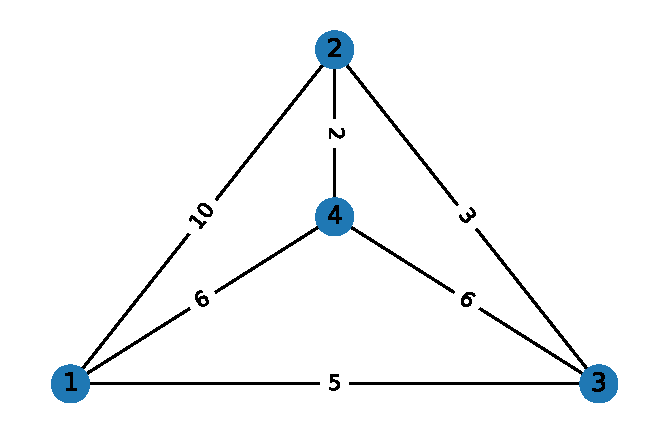
\includegraphics{index_files/figure-pdf/fig-shortest-path-sparsification-output-1.pdf}

}

}

\subcaption{\label{fig-shortest-path-sparsification-1}The graph \(G\)
that we intend to sparsify.}
\end{minipage}%
%
\begin{minipage}[t]{0.50\linewidth}

{\centering 

\raisebox{-\height}{

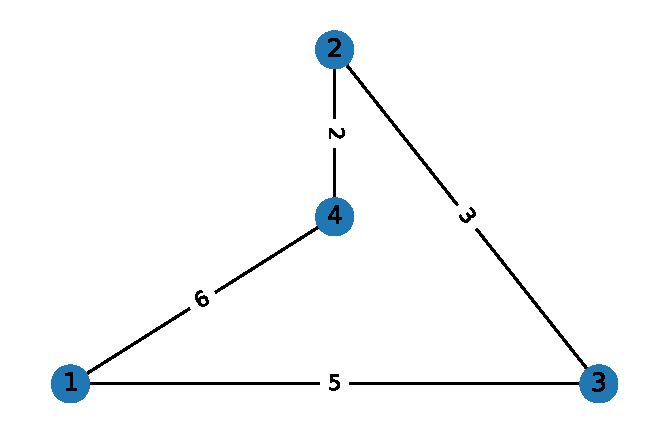
\includegraphics{index_files/figure-pdf/fig-shortest-path-sparsification-output-2.pdf}

}

}

\subcaption{\label{fig-shortest-path-sparsification-2}The graph \(H\)
that is obtained by removing trivial edges.}
\end{minipage}%

\caption{\label{fig-shortest-path-sparsification}A simple illustration
of a sparsifier that can help with shortest path problems.}

\end{figure}

On the other hand, (Benczúr and Karger 1996) for example introduces the
cut-sparsifiers which are a class of sparsifiers that have almost
identical cut weights for any set \(S \subset V\). In this report, we
cover spectral graph sparsifiers which are a certain class of
sparsifiers that have a tight connection with expander graphs and can
approximate the Laplacian of a graph with high accuracy. Because of the
close connection between graph spectral connectivity and edge
connectivity introduced by Cheeger (Cheeger 1970) spectral sparsifiers
were introduced by (Spielman and Teng 2004) and (Spielman and Teng
2011). Conventionally, these graphs are constructed using randomized
algorithms where we pick a certain edge of an original graph with a
probability. For example, if an edge is crucial to the connectivity of
our graph, then it has high importance and should be picked with high
probability. However, in this report, we will show that we can construct
a sparsifier with a deterministic algorithm introduced in (Batson,
Spielman, and Srivastava 2009) that has a tight connection with the
Ramanujan bounds.

Furthermore, we will cover an important reduction from the graph
sparsification problem to a matrix approximation problem which has been
further exploder in many follow-up papers (Tat Lee and Sun 2015) and
(Lee and Sun 2017). Moreover, this will give us the first deterministic
algorithm for obtaining sparsifiers with linear edge count. That said,
we have implemented the algorithm in Python and have tested it on a few
graphs for illustration purposes.

Finally, we will focus our attention on running the algorithm on
complete graphs. The sparsifier obtained from the complete graph will
have high connectivity which resembles similarities with the expander
graphs. Although the graph obtained from the algorithm is not regular,
we will show that it has a lot of expander-like properties and we will
draw a close connection with Ramanujan graphs.

\hypertarget{recap-and-preliminaries}{%
\subsection{Recap and Preliminaries}\label{recap-and-preliminaries}}

Here we will cover some preliminaries on spectral sparsification and
then we will discuss the effective resistance-based algorithm for
spectral sparsification. We will also discuss an important reduction to
the matrix problem that was first formalized in (Batson, Spielman, and
Srivastava 2009) which lays the groundwork for the final algorithm.

\hypertarget{spectral-sparsification}{%
\subsubsection{Spectral Sparsification}\label{spectral-sparsification}}

Before everything, we should define what a spectral sparsifier is. A
spectral sparsifier is a sparse graph that approximates the Laplacian of
a graph with high accuracy. In other words, a sparsifier is a graph that
has a lot of the same properties as the original graph.

\leavevmode\vadjust pre{\hypertarget{def-spectral-sparsification}{}}%
\begin{definition}[]\label{def-spectral-sparsification}

A \((k, \epsilon)\)-spectral sparsifier of a graph \(G = (V, E, w)\) is
a graph \(H\) with \(k\) edges such that,
\[L_G \approx_\epsilon L_H : (1 - \epsilon) L_G \preceq L_H \preceq (1 + \epsilon) L_G\]
where \(L_G\) is the Laplacian of \(G\) and \(L_H\) is the Laplacian of
\(H\).

\end{definition}

\hypertarget{reduction-to-the-matrix-problem}{%
\subsubsection{Reduction to the Matrix
Problem}\label{reduction-to-the-matrix-problem}}

Here, we will present an analog problem for the sparsification of
matrices that is tightly connected to the spectral sparsification
problem. The problem is as follows:

\leavevmode\vadjust pre{\hypertarget{def-matrix-approximation}{}}%
\begin{definition}[]\label{def-matrix-approximation}

\textbf{\((k, \epsilon)\)-approximation of matrices} Given a set of
\(m\) vectors \(v_1, \ldots, v_m \in \mathbb{R}^n\) if
\(A = \sum_{i=1}^m v_iv_i^T\) is a positive semi-definite matrix, then
we intend to find a subset of vectors
\(\mathcal{S} \subseteq \{1, \ldots, m\}\) of size \(k\) and a set of
coefficients \(s_i \in \mathbb{R}^+\) such that
\(\hat{A} = \sum_{i \in \mathcal{S}} s_i v_i v_i^T \approx_\epsilon A\).

\end{definition}

Now we will show that one can solve the \((k, \epsilon)\) problem in
Definition~\ref{def-matrix-approximation} then it can plug into the
graph sparsification problem and obtain a \((k, \epsilon)\)-spectral
sparsifier. To do so, observe that if we set \(A = L_G\) and
\(v_{ab} = \sqrt{w_G(a,b)} (\chi_a - \chi_b)\) and
\(s_{ab} = \frac{w_H(a,b)}{w_G(a,b)}\), then the problem in
Definition~\ref{def-matrix-approximation} is equivalent to the spectral
sparsification problem:

\begin{align*}
A = L_G &= \sum_{(a,b) \in E(G)} w_G(a,b) L_{ab} \\
&= \sum_{(a,b) \in E(G)} \sqrt{w_G(a,b)}^2 (\chi_a - \chi_b) (\chi_a - \chi_b)^T\\
& = \sum_{ab \in E(G)} v_{ab} v_{ab}^T\\
\hat{A} = L_H &= \sum_{(a, b) \in E(H)} w_H(a,b) L_{ab} \\
&= \sum_{(a, b) \in E(H)} \frac{w_H(a,b)}{w_G(a,b)} \sqrt{w_G(a,b)}^2 (\chi_a - \chi_b) (\chi_a - \chi_b)^T\\
&= \sum_{(a,b) \in E(H)} s_{ab} v_{ab} v_{ab}^T
\end{align*}

\hypertarget{sampling-based-sparsification}{%
\subsubsection{Sampling-based
Sparsification}\label{sampling-based-sparsification}}

As alluded to previously, the problem of spectral sparsification can be
approached from an edge-sampling perspective. In particular, one can
assign importance weights to each edge and then come up with a sampling
scheme that samples edges according to their importance. For example, an
edge that is crucial for the connectivity of the graph has high
importance for cut-sparsifiers or spectral sparsifiers. To that end, a
set of edges can be independently sampled according to this scheme and
after sampling each edge the graph becomes more and more similar to the
original graph. However, since this sampling is done according to the
measure of importance, even after sampling a small number of edges, the
graph becomes a good approximation of the original graph.

One can also formulate the same thing for the matrix approximation
problem. Assume that for each vector \(i\), we have a corresponding
matrix \(X_i = s_i v_i v_i^T\) which will be picked with probability
\(p_i\) and we will consider \(\hat{A} = \sum_{i \in \mathcal{S}} X_i\)
where \(\mathcal{S}\) is the set of indices of the sampled vectors. One
can bound the number of sampled vectors by coming up with good
probabilities \(p_i\) such that \(\sum p_i\) is bounded by \(k\) and can
also bound the error of the approximation by using matrix concentration
bounds. However, these algorithms tend to have the following problems:

\begin{enumerate}
\def\labelenumi{\arabic{enumi}.}
\tightlist
\item
  The algorithm is not deterministic meaning that there is a very low
  chance of producing a large set \(\mathcal{S}\).
\item
  The algorithm is not deterministic meaning that there is a very low
  chance of producing an approximate \(\hat{A}\) which is not close to
  \(A\).
\item
  Because these algorithms rely on exponential concentration bounds,
  typically they require to sample \(\mathcal{O}(n \cdot polylog(n))\)
  vectors to achieve a good approximation.
\end{enumerate}

Although flawed, these solutions are easy and using this idea, a set of
sampling techniques have been proposed to tackle the problem of
sparsification with the most famous among them being the
\textbf{effective-resistance} based sparsifiers (Spielman and Srivastava
2008). We will briefly cover the main idea and intuition behind this and
redirect the reader to other resources for further detailed reading.

The effective resistance between two nodes \(a\) and \(b\) is the
equivalent resistance if we assume that the rest of the nodes are
harmonic and only one external current is given to \(a\) and one
external current is taken from \(b\); then, the measured voltage
difference between these two nodes will denote the effective resistance
which can be written as \((\chi_a - \chi_b)^T L^+_G (\chi_a - \chi_b)\)
using Laplacians. Moreover, effective resistances have a combinatorial
interpretation as well. If we assume we sample spanning trees
proportional to their weight products, then the effective resistance
between two nodes is proportional to the probability of the edge between
those two nodes appearing. This means that a crucial edge in the
connectivity, will have a high probability of appearing in the sampled
spanning trees and thus will have a high effective resistance; that
said, this will yield a high importance weight for that edge and thus it
will be sampled more often:

\textbf{Effective-resistance based sparsifier} For each edge
\((a, b) \in E\), sample \((a,b)\) with probability
\(p(a,b) = \min\left(1, C\cdot (\log n) \epsilon^{-2} w(a,b) R_{eff}(a, b)\right)\).
Where \(R_{eff}(a, b)\) is the effective resistance between \(a\) and
\(b\). Using Rudelson concentration lemma (Rudelson 1999), (Spielman and
Srivastava 2008) shows that for a certain constant \(C\) after picking
\(\mathcal{O}(n\log n /\epsilon)\) edges the resulting graph is a
\(\epsilon\)-spectral sparsifier with high probability.

\hypertarget{method}{%
\subsection{Method}\label{method}}

We will now discuss the deterministic algorithm for approximating the
matrix \(A\). The algorithm takes an iterative approach and follows
\(k\) iterations. At each iteration, it will pick a vector \(v_i\) which
corresponds to an edge and will add \(s_i v_i v_i^T\) to the current
accumulated matrix. After \(k\) iterations it will give a good
approximate for the matrix \(A\). But before we present the bulk of the
algorithm, let's start by laying some groundwork by presenting some
useful intuitions.

\hypertarget{geometric-interpretation}{%
\subsubsection{Geometric
interpretation}\label{geometric-interpretation}}

Note that for any pair of matrices \(A\) and \(B\), having the same
null-space we have that
\(A \succeq B \Longleftrightarrow I \succeq A^{+/2} B A^{+/2}\). Hence,
\[(1 - \epsilon) A \approx_\epsilon B \Longleftrightarrow \Pi \approx_\epsilon A^{+/2} B A^{+/2}\]
where \(\Pi = A^{+/2} A A^{+/2}\) is the identity in the subspace
orthogonal to the null space of \(A\) and is an \emph{idempotent}
matrix. In other words, \(\Pi^2 = \Pi\). Therefore, without loss of
generality, we may assume that \(A\) in
Definition~\ref{def-matrix-approximation} is an idempotent matrix
\(\Pi\) via the transformation described where \(A\) is replaced by
\(A^{+/2} A A^{+/2}\) and \(v_i = A^{+/2} v_i\) for all
\(1 \le i \le m\).

With that in mind, thinking about idempotent matrices yields nice
intuitions on how to think about the problem geometrically. Furthermore,
for any positive semi-definite matrix \(M\) we can define an ellipsoid
\(\{x | x^T M x = 1\}\) and for \(M = \Pi\) being an idempotent matrix
the ellipsoid corresponds to the sphere in the linearly transformed
subspace of \(\Pi\): \[x^T \Pi x = x^T \Pi \Pi x = ||\Pi x||_2^2 = 1.\]

Therefore, if we consider everything in the mapped subspace, i.e.,
replacing every vector \(x\) with \(\Pi x\) automatically, then we want
to find a linear combination of their cross product such that the
ellipsoid corresponding to that combination approximates a regular
spherical shape. In other words, \begin{align*}
&\hat{A} = \sum s_i v_i v_i^T \approx_\epsilon A \\
\Longleftrightarrow & ~ \hat{\Pi} = \sum s_i (A^{+/2}) v_i (A^{+/2} v_i)^T  \approx_\epsilon A^{+/2} A A^{+/2} = \Pi\\
\Longleftrightarrow & ~ (1 - \epsilon) \Pi \preceq \hat{\Pi} \preceq (1 + \epsilon) \Pi \\
\Longleftrightarrow & ~ \forall x : (1 - \epsilon) ||\Pi x||_2^2 \le [\Pi x]^T \hat{\Pi} [\Pi x] \le (1 + \epsilon) ||\Pi x||_2^2 \\
\end{align*}

Therefore, the ellipsoid projected using \(\Pi\) is sandwiched between
two spheres off by \(\epsilon\) in their radius. Therefore, the
algorithm takes an iterative approach to solve this geometric problem.
It first starts of with \(\hat{A}^{(0)} = \emptyset\) and then
iteratively picks a vector \(v_i\) and assigns a weight \(s_i\) to it
such that the ellipsoid
\(\hat{A}^{(i)} = \hat{A}^{(i+1)} + s_i v_i v_i^T\) becomes iteratively
more like a sphere. To formalize this, the algorithm always bounds the
corresponding ellipsoid between two spheres of radius \(l^{(i)}\) and
\(u^{(i)}\). At the beginning of each iteration, the lower bound
\(l^{(i)}\) will be increased by some \(\delta_l\) and the lower bound
\(u^{(i)}\) will be increased by some \(\delta_u\) and the algorithm
will try to find a vector \(v_i\) and a weight \(s_i\) such that the new
ellipsoid \(\hat{A}^{(i+1)}\). Moreover, the key idea here is to
cleverly pick \(\delta_l\) and \(\delta_u\) values such that after \(k\)
iterations the gap between the two spheres is off by \(\epsilon\). In
other words, the following should hold:
\[\frac{u^{(0)} + k \delta_u}{l^{(k)} + k \delta_l} = \frac{u^{(k)}}{l^{(k)}} \le \frac{1 + \epsilon}{1 - \epsilon}.\]
This will ensure that the shape of the ellipsoid becomes more and more
spherical as the algorithm progresses, and finally, a simple scaling
will yield an approximate unit sphere which is what we want.

For illustration, the following shows the algorithm in action. The
algorithm starts with an initial ellipsoid that is not spherical and
then iteratively picks a vector \(v_i\) and a weight \(s_i\) such that
it still remains sandwiched between two spheres of radius \(l^{(i)}\)
and \(u^{(i)}\). Note that in this example \(\delta_l\) and \(\delta_u\)
are equal, therefore, for a large enough \(k\) the ellipsoid will become
spherical because although the radius is growing the gap remains the
same, further limiting the range of the ellipsoid.

\hypertarget{physical-view-and-the-expected-behavior}{%
\subsection{Physical View and the Expected
behavior}\label{physical-view-and-the-expected-behavior}}

The fact that \(\hat{A}^{(i)}\) should be bounded between two spheres
translates into all the eigenvalues of \(\hat{A}^{(i)}\) being bounded
between the two radiuses. Therefore, an important observation is to
monitor what happens to the eigenvalues of \(\hat{A}^{(i)}\) when
\(vv^T\) is being added at each iteration. To do so, we consider the
characteristic polynomial of \(A\) at each iteration written as
\(p_A(\lambda) = \det(\lambda I - A)\). There are two important lemmas
when analyzing \(A + vv^T\) matrices, one is the Sherman-Morrison lemma
which states that:

\leavevmode\vadjust pre{\hypertarget{lemma-sherman-morrison}{}}%
Suppose \(A\) is an invertible square matrix and \(u, v\) are column
vectors. Then \(A + uv^T\) is invertible iff
\(1 + v^T A^{-1} u \neq 0\). In this case,
\[(A + uv^T)^{-1} = A^{-1} - \frac{A^{-1}uv^TA^{-1}}{1 + v^TA^{-1}u}\]

The other is the matrix determinant lemma which states that:

\leavevmode\vadjust pre{\hypertarget{lemma-matrix-determinant}{}}%
Suppose \(A\) is an invertible square matrix and \(u, v\) are column
vectors. Then \[\det(A + uv^T) = \det(A) (1 + v^T A^{-1} u)\]

Moreover, plugging these into the characteristic polynomial of
\(A + vv^T\) yields the following:

\begin{align*}
p_{A + vv^T}(\lambda) &= \det(\lambda I - A - vv^T) \\
& = \det(\lambda I - A) (1 - v^T \left(\lambda I - A \right)^{-1}u) \\
& = \det (\lambda I - A) \left(1 - v^T \left[\sum_{i=1}^n \frac{1}{\lambda - \lambda_i} u_i u_i^T\right] v\right)\\
& = p_A(\lambda) \left(1 -  \sum_{i=1}^n \frac{(v^Tu_i)^2}{\lambda - \lambda_i}\right)\\
\end{align*}

Therefore, we can assume particles being set on each of the
\(\lambda_i\) values with the \(i\)th one on \(\lambda_i\) with charge
\(v^Tu_i\). The new set of equilibrium points for this particle set will
entail the new eigenvalues of \(A + vv^T\) which are the roots of
\(p_{A + vv^T}(\lambda)\). Note that for \(u_i\) values such that
\(v^Tu_i=0\) the charge is zero and therefore, the new eigenvalues will
be the same as the old ones.

The following figure illustrates the matrix case \(A\) with three
different vectors \(v_1\), \(v_2\) and \(v_3\). Each color corresponds
to the characteristic polynomial for different \(v\) values where,

\[A = \lambda_1 u_1 u_1^T + \lambda_2 u_2 u_2^T + \lambda_3 u_3 u_3^T
 = \begin{bmatrix}
1.6 & -0.2 & -0.33\\
-0.2 & 3.4 & -0.33\\
-0.33 & -0.33 & 1
\end{bmatrix}\]
\[\begin{bmatrix}\lambda_1 \\ \lambda_2 \\ \lambda_3\end{bmatrix} = \begin{bmatrix}0.79 \\ 1.75 \\ 3.46\end{bmatrix}, u_1 = \begin{bmatrix}
-0.41\\
-0.15\\
-0.9
\end{bmatrix}, u_2 = \begin{bmatrix}
-0.9 \\
-0.03 \\
0.42
\end{bmatrix}, u_3 = \begin{bmatrix}
0.08\\
-0.99\\
0.12\\
\end{bmatrix}\] We note that \(\langle v_i, u_j \rangle^2\) is the
charge of particle \(j\) when adding \(v_i\) to \(A\) and we can
summarize all the charged particles in the following matrix:
\[v_1 = \begin{bmatrix}
0\\
1\\
1\\
\end{bmatrix}, v_2 = \begin{bmatrix}
1\\
1\\
0\\
\end{bmatrix}, 
C = \begin{bmatrix}
1.10 & 0.15 & 0.75\\
0.31 & 0.87 & 0.82
\end{bmatrix}, C_{ij} = \langle v_i, u_j \rangle^2\]

\begin{Shaded}
\begin{Highlighting}[]
\ImportTok{import}\NormalTok{ numpy }\ImportTok{as}\NormalTok{ np}
\ImportTok{import}\NormalTok{ matplotlib.pyplot }\ImportTok{as}\NormalTok{ plt}

\KeywordTok{def}\NormalTok{ plot\_characteristic\_polynomial(A, v, color):}
\NormalTok{  x }\OperatorTok{=}\NormalTok{ np.linspace(}\OperatorTok{{-}}\DecValTok{25}\NormalTok{, }\DecValTok{50}\NormalTok{, }\DecValTok{1000}\NormalTok{)}
\NormalTok{  w, u }\OperatorTok{=}\NormalTok{ np.linalg.eig(A)}
  \CommentTok{\# plot the determinant of xI {-} A}
\NormalTok{  y }\OperatorTok{=}\NormalTok{ []}
\NormalTok{  roots }\OperatorTok{=}\NormalTok{ []}
\NormalTok{  prv }\OperatorTok{=} \DecValTok{0}
  \ControlFlowTok{for}\NormalTok{ i }\KeywordTok{in}\NormalTok{ x:}
\NormalTok{    val }\OperatorTok{=} \DecValTok{1} \OperatorTok{{-}}\NormalTok{ np.}\BuiltInTok{sum}\NormalTok{(}\DecValTok{1}\OperatorTok{/}\NormalTok{(i }\OperatorTok{{-}}\NormalTok{ w) }\OperatorTok{*}\NormalTok{ (v }\OperatorTok{@}\NormalTok{ u)}\OperatorTok{**}\DecValTok{2}\NormalTok{)}
    \ControlFlowTok{if}\NormalTok{ prv }\OperatorTok{\textless{}} \DecValTok{0} \KeywordTok{and}\NormalTok{ val }\OperatorTok{\textgreater{}} \DecValTok{0}\NormalTok{:}
\NormalTok{      roots.append(i)}
\NormalTok{    prv }\OperatorTok{=}\NormalTok{ val}
\NormalTok{    y.append(val)}
\NormalTok{  plt.plot(x, y, color }\OperatorTok{=}\NormalTok{ color, label}\OperatorTok{=}\StringTok{\textquotesingle{}characteristic polynomial of A + vv\^{}T\textquotesingle{}}\NormalTok{)}
\NormalTok{  plt.scatter(roots, np.zeros(}\BuiltInTok{len}\NormalTok{(roots)), color }\OperatorTok{=}\NormalTok{ color, marker }\OperatorTok{=} \StringTok{\textquotesingle{}o\textquotesingle{}}\NormalTok{, label}\OperatorTok{=}\StringTok{\textquotesingle{}new{-}eigenvalues\textquotesingle{}}\NormalTok{)}

\CommentTok{\# create an orthonormal 3 by 3 matrix U}
\NormalTok{U }\OperatorTok{=}\NormalTok{ np.array([[}\DecValTok{1}\NormalTok{, }\DecValTok{1}\NormalTok{, }\DecValTok{1}\NormalTok{], [}\DecValTok{1}\NormalTok{, }\DecValTok{1}\NormalTok{, }\OperatorTok{{-}}\DecValTok{2}\NormalTok{], [}\DecValTok{1}\NormalTok{, }\OperatorTok{{-}}\DecValTok{1}\NormalTok{, }\DecValTok{0}\NormalTok{]])}
\NormalTok{U }\OperatorTok{=}\NormalTok{ U }\OperatorTok{/}\NormalTok{ np.linalg.norm(U, axis }\OperatorTok{=} \DecValTok{0}\NormalTok{)}
\NormalTok{A }\OperatorTok{=}\NormalTok{ U }\OperatorTok{@}\NormalTok{ np.diag([}\DecValTok{1}\NormalTok{ , }\DecValTok{2}\NormalTok{, }\DecValTok{3}\NormalTok{]) }\OperatorTok{@}\NormalTok{ U.T}



\NormalTok{vz }\OperatorTok{=}\NormalTok{ [[}\DecValTok{0}\NormalTok{, }\DecValTok{1}\NormalTok{, }\DecValTok{1}\NormalTok{], [}\DecValTok{1}\NormalTok{, }\DecValTok{1}\NormalTok{, }\DecValTok{0}\NormalTok{]]}

\NormalTok{colors }\OperatorTok{=}\NormalTok{ [}\StringTok{\textquotesingle{}blue\textquotesingle{}}\NormalTok{, }\StringTok{\textquotesingle{}red\textquotesingle{}}\NormalTok{]}

\CommentTok{\# plot the eigenvalues of A}
\NormalTok{w, u }\OperatorTok{=}\NormalTok{ np.linalg.eig(A)}
\CommentTok{\# sort according to w and reorder u}
\NormalTok{w, u }\OperatorTok{=} \BuiltInTok{zip}\NormalTok{(}\OperatorTok{*}\BuiltInTok{sorted}\NormalTok{(}\BuiltInTok{zip}\NormalTok{(w, u.T)))}
\NormalTok{u }\OperatorTok{=}\NormalTok{ np.array(u).T}
\NormalTok{w }\OperatorTok{=}\NormalTok{ np.array(w)}

\ControlFlowTok{for}\NormalTok{ col, v }\KeywordTok{in} \BuiltInTok{zip}\NormalTok{(colors, vz):}
\NormalTok{  plt.scatter(w, np.zeros(w.shape), color }\OperatorTok{=} \StringTok{\textquotesingle{}black\textquotesingle{}}\NormalTok{, marker }\OperatorTok{=} \StringTok{\textquotesingle{}x\textquotesingle{}}\NormalTok{, label}\OperatorTok{=}\StringTok{\textquotesingle{}previous eigenvalues\textquotesingle{}}\NormalTok{)}
  \CommentTok{\# add text with textbox equal to np.sum(w) on top of each eigenvalue}
  \ControlFlowTok{for}\NormalTok{ i, wi }\KeywordTok{in} \BuiltInTok{enumerate}\NormalTok{(w):}
\NormalTok{    t }\OperatorTok{=}\NormalTok{ plt.text(wi }\OperatorTok{{-}} \FloatTok{0.5}\NormalTok{, }\FloatTok{0.1} \OperatorTok{*}\NormalTok{ (}\DecValTok{4} \OperatorTok{*}\NormalTok{ (i }\OperatorTok{\%} \DecValTok{2}\NormalTok{) }\OperatorTok{{-}} \FloatTok{2.5}\NormalTok{), }\SpecialStringTok{f"c=}\SpecialCharTok{\{}\NormalTok{(v }\OperatorTok{@}\NormalTok{ u[:,i])}\OperatorTok{**}\DecValTok{2}\SpecialCharTok{:.2f\}}\SpecialStringTok{"}\NormalTok{, color }\OperatorTok{=} \StringTok{\textquotesingle{}black\textquotesingle{}}\NormalTok{)}
\NormalTok{    t.set\_bbox(}\BuiltInTok{dict}\NormalTok{(facecolor}\OperatorTok{=}\StringTok{\textquotesingle{}white\textquotesingle{}}\NormalTok{, alpha}\OperatorTok{=}\FloatTok{0.5}\NormalTok{, edgecolor}\OperatorTok{=}\NormalTok{col))}

\NormalTok{  plot\_characteristic\_polynomial(A, v, col)}
\NormalTok{  plt.xlim(}\DecValTok{0}\NormalTok{, }\FloatTok{5.5}\NormalTok{)}
\NormalTok{  plt.ylim(}\OperatorTok{{-}}\DecValTok{2}\NormalTok{, }\DecValTok{2}\NormalTok{)}
\NormalTok{  plt.legend()}
\NormalTok{  plt.show()}
\end{Highlighting}
\end{Shaded}

\begin{figure}

\begin{minipage}[t]{0.50\linewidth}

{\centering 

\raisebox{-\height}{

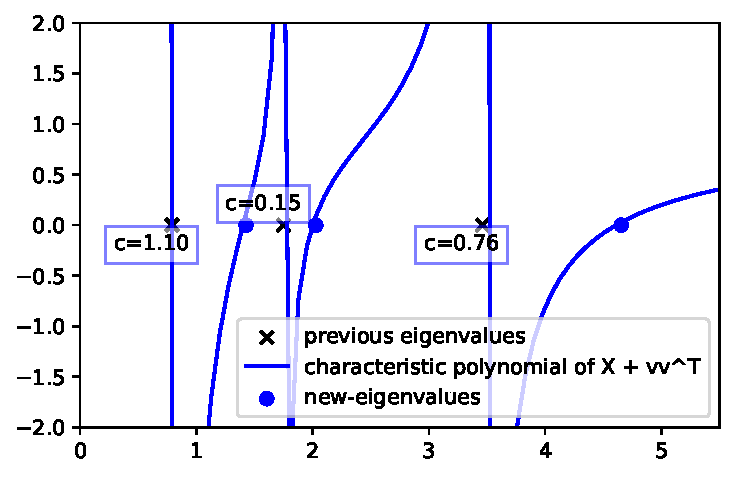
\includegraphics{index_files/figure-pdf/fig-matrix-determinant-output-1.pdf}

}

}

\subcaption{\label{fig-matrix-determinant-1}The characteristic
polynomial after adding \(v_1\) to A.}
\end{minipage}%
%
\begin{minipage}[t]{0.50\linewidth}

{\centering 

\raisebox{-\height}{

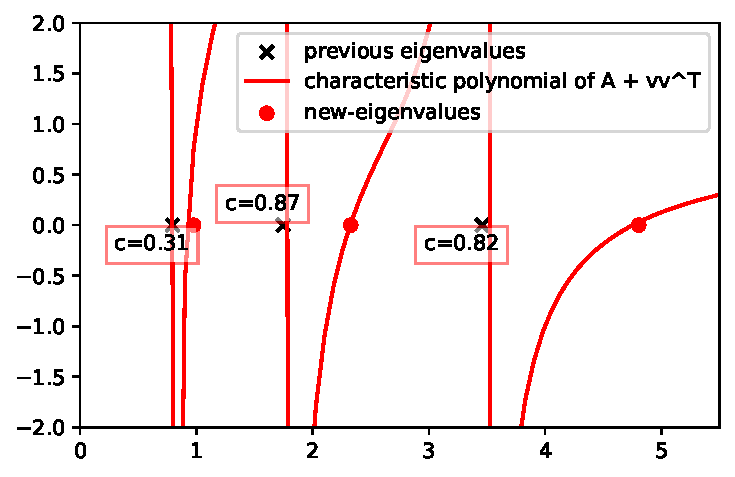
\includegraphics{index_files/figure-pdf/fig-matrix-determinant-output-2.pdf}

}

}

\subcaption{\label{fig-matrix-determinant-2}The characteristic
polynomial after adding \(v_2\) to A.}
\end{minipage}%

\caption{\label{fig-matrix-determinant}The characteristic polynomial of
\(A + vv^T\) for different \(v\) values, the higher the charge the more
it will repel the new eigenvalues from the old ones.}

\end{figure}

The goal is to pick a \(v\) such that all the eigenvalues are uniformly
pushed forward so that they can stay between the new ranges
\(l^{(i+1)}\) and \(u^{(i+1)}\). To get a sense, let's pick one of the
\(m\) vectors with uniform probability and add it to \(A\). In that
case, the expected charges can be written as:
\[E[\langle v, u_j \rangle^2] = \frac{1}{m} \sum_{i=1}^m \langle v_i, u_j \rangle^2 = \frac{1}{m} u_j^T \left( \sum_{i=1}^m v_i v_i^T \right)u_j = \frac{||\Pi u_j||_2^2}{m} = \frac{1}{m}\]
Hence, on expectation all the particles have charge \(1/m\) and the
expected deterministic polynomial is:

\begin{align*}
E[p_{A + v}(\lambda)] &= p_A(\lambda) E\left[1 - \sum_{i=1}^m \frac{\langle u_i, v\rangle^2}{\lambda - \lambda_i}\right] = p_A(\lambda) \left(1 - \sum_{i=1}^m \frac{E\langle u_i, v\rangle^2}{\lambda - \lambda_i}\right)\\
& = p_A(\lambda) \left(1 - \sum_{i=1}^m \frac{1/m}{\lambda - \lambda_i}\right) = p_A(\lambda) - \frac{1}{m} \sum_{i=1}^m \frac{p_A(\lambda)}{\lambda - \lambda_i}\\
& = p_A(\lambda) - \frac{1}{m} \sum_{i=1}^m \prod_{1 = j\neq i}^m (\lambda - \lambda_j)\\
&= p_A(\lambda) - \frac{1}{m} p'_A(\lambda)\\
\end{align*}

Therefore, if we start off with the matrix
\(p_{A^{(0)}}(\lambda) = \lambda^n\), after \(nd\) iterations the
expected polynomial is a set of associate Laguerre polynomials that are
well studied (Dette and Studden 1995), and in particular, it has been
proven that the ratio between the largest and smallest root for these
polynomials is bounded by the value below:

\[\frac{d + 1 + 2\sqrt{d}}{d + 1 - 2\sqrt{d}} \xrightarrow{\epsilon = \frac{2\sqrt{d}}{d+1}} \frac{1 + \epsilon
}{1 - \epsilon}\]

Although this is just speculation and no \(v_i\) values will necessarily
exist with the expected behavior, we can still get an idea of the goal
\(\epsilon\) and come up with the following proposition:

\leavevmode\vadjust pre{\hypertarget{prp-final-form}{}}%
\begin{proposition}[]\label{prp-final-form}

For any matrix \(A = \sum_{i=1}^m v_i v_i^T\) we can choose a subset
\(\mathcal{S}\) of \(v_i\) and a set of coefficients \(s_i\) with size
\(nd\) such that:
\[\hat{A} = \sum_{i \in \mathcal{S}} s_i \cdot v_i v_i^T,~~ (1 - \frac{2\sqrt{d}}{d+1}) A \preceq \hat{A} \preceq (1 + \frac{2\sqrt{d}}{d+1}) A\]

\end{proposition}

The graph formulation of Proposition~\ref{prp-final-form} is as follows:

\leavevmode\vadjust pre{\hypertarget{cor-final-form}{}}%
\begin{corollary}[]\label{cor-final-form}

For any graph \(G\) and any \(\epsilon\) we can choose a subset of
\(\mathcal{O}(n/\epsilon^2)\) edges with arbitrary edge weights to
obtain \(H\) such that \(H\) is an \(\epsilon\)-sparsifier of \(G\):
\(L_G \approx_\epsilon L_H\).

\end{corollary}

This is set using \(\epsilon = \frac{2\sqrt{d}}{d + 1}\) where
\(\frac{n}{\epsilon^2} = \mathcal{O}(nd)\). In the next section, we will
see how we can choose \(v_i\) and \(s_i\) at each step such that after
\(nd\) iterations this happens.

\hypertarget{potential-functions}{%
\subsubsection{Potential Functions}\label{potential-functions}}

The big question is, how can we quantize the boundedness of the matrix
\(A\) at each step? We want \(A^{(i)}\) to have eigenvalues that are
bounded by \(l^{(i+1)}\) and \(u^{(i+1)}\); and so, we use a family of
\textbf{potential functions} that explode when the eigenvalues approach
the bounds. A set of such potentials can be chosen using the fact that
\(uI - A\) or \(A - lI\) will have infinitely small eigenvalues when the
eigenvalues of \(A\) approach \(u\) or \(l\) respectively; therefore,
their inverse will be ill-conditioned and have infinitely large
eigenvalues. We can use the following potential functions:

\[\Phi^u_l(A) = \Phi^u(A) + \Phi_l(A) = Tr[(uI - A)^{-1}] + Tr[(A - l I)^{-1}]\]

In summary, the main idea is to choose \(v_i\) and \(s_i\) such that the
potential for the matrix \(A^{(i)}\) in the next iteration does not
explode. To do so, we ensure that the potentials remain monotonically
decreasing:

\[\infty \gg \Phi^{u^{(0)}}(A^{(0)}) \ge \Phi^{u^{(1)}}(A^{(1)}) \ge ... \ge \Phi^{u^{(nd)}}(A^{(nd)})\]
\[\infty \gg \Phi_{\ell^{(0)}}(A^{(0)}) \ge \Phi_{\ell^{(1)}}(A^{(1)}) \ge ... \ge \Phi_{\ell^{(nd)}}(A^{(nd)})\]

With that in mind, let's assume we are going to assign \(s_k\) to any
vector \(v_k\) such that after the increase in our upper and lower
bound, the potential remains non-increasing. Now let us separately
consider the upper and lower bound potentials.

When increasing \(l^{(i)}\), the eigenvalues come closer to the lower
bound, and hence, the potential of the lower bound will increase;
therefore, for any vector \(v_k\), the coefficient \(s_k\) should be
bounded by some value \(L_{A^{(i)}}(v_k)\) such that after adding
\(s_k \cdot v_k v_k^T\) to \(A^{(i)}\), spectrum shifts forward and the
increase in the potential cancels out. That said, for any matrix \(A\)
and any vector \(v\) we have:

\begin{align*}
&\Phi^{\overset{l'}{\overbrace{l + \delta_l}}}(A + s \cdot vv^T) \le \Phi^l(A)\\
\Phi_{l'}(A + s \cdot vv^T) & = Tr(A + s \cdot vv^T - l'I)^{-1}  \qquad \text{Sherman-Morrison}\\\
& = Tr\left((A - l'I)^{-1}\right) + Tr\left(\frac{s \cdot (A - l'I)^{-1} v v^T (A - l'I)^{-1}}{1 + s \cdot v^T (A - l' I)^{-1} v}\right)\\
&= \Phi_{l'}(A) - \frac{s \cdot v^T (A - l'I)^{-2}v}{1 + s \cdot v^T  (A - l'I)^{-1}v} \le \Phi^l(A)\\
\Leftrightarrow &~ \underset{\Delta}{\underbrace{\Phi_{l'}(A) - \Phi^l(A)}} \le \frac{s \cdot v^T (A - l'I)^{-2}v}{1 + s \cdot v^T  (A - l'I)^{-1}v}\\
\Leftrightarrow &~ s\cdot \left[v^T (A - l'I)^{-2}v  - \Delta v^T(A - l' I)^{-1} v\right] \ge \Delta\\
\Leftrightarrow &~ s \ge \frac{\Delta}{v^T \left( (A - l'I)^{-2} - \Delta (A - l' I)^{-1} \right) v} = L_A(v)
\end{align*}row \&\textasciitilde{} s
\ge \frac{\Delta}{v^T \left( (A - l'I)^{-2} - \Delta (A - l' I)^{-1} \right) v}
= L\_A(v) \textbackslash end\{align*\}

which means,

\begin{equation} \tag{1}\label{eq:lower-bound-potential}
s \ge L_A(v) = \frac{\Delta}{v^T \left((A - l' I)^{-2} - \Delta (A - l' I)^{-1} \right) v}
\end{equation}

On the other hand, a similar thing can be said for the upper-bound
potential. when increasing \(u^{(i)}\), the eigenvalues are further away
from the upper bound which gives us the freedom to shift the eigenvalues
forward. However, this shifting should not be so extreme that the
potential at most increases offset the decrease introduced after adding
\(\delta_u\) to the potential.

\[ 
\Phi^{\overset{u'}{\overbrace{u + \delta_u}}}(A + s \cdot vv^T) \le \Phi^u(A)
\]

Similar to \(\eqref{eq:lower-bound-potential}\), if we negate \(s\) and
\(A\) then the upper-bound potential will act similarly to the
lower-bound potential. Therefore, we can write the following:

\begin{equation} \tag{2}\label{eq:upper-bound-potential}
s \le U_A(v) = \frac{\Delta}{v^T \left((u' I - A)^{-2} - \Delta (u' I - A)^{-1}\right)v}
\end{equation}

Where \(\Delta\) is the difference between \(\Phi^u(A)\) and
\(\Phi^{u'}(A)\).

Finally, for every vector \(v_i\) at each step, we can introduce an
upper and lower bound for the coefficient corresponding to that vector.
However, this is not enough to ensure that at least one \(v_i\) exists
such that \(L_A\); in other words, it might be the case that for each
vector the upper and lower bounds are contradictory which will put the
algorithm in a stale-mate state. To avoid this, we pick the values
\(\delta_u\) and \(\delta_l\) carefully and introduce a nice lemma in
the next section that ensures always such a vector exists.

\hypertarget{the-existence-of-a-good-vector}{%
\subsubsection{The Existence of a good
Vector}\label{the-existence-of-a-good-vector}}

We will now present the following lemma, that for the potentials having
a certain condition, a good vector \(v_k\) and a good coefficient
\(s_k\) always exist. This is the meat and bones of the algorithm:

\leavevmode\vadjust pre{\hypertarget{lem-good-vector-existance}{}}%
\begin{lemma}[]\label{lem-good-vector-existance}

For any set of vectors \(\langle v_1, v_2, ..., v_m \rangle\) that sum
up to an idempotent matrix \(\Pi = \sum v_i v_i^T\) and a matrix \(A\)
being an arbitrary linear combination of their rank one cross product,
if \(\Phi^u(A) \le \epsilon_U\) and \(\Phi_l(A) \le \epsilon_L\) and
\(\epsilon_u, \epsilon_l, \delta_u, \delta_l\) satisfy the following
conditions:
\[0 \le \delta_u^{-1} + \epsilon_u \le \delta_l^{-1} - \epsilon_l,\]
Then, there exists a vector \(v_k\) such that: \[L_A(v_k) \le U_A(v_k)\]
, and hence, by adding an \(A\) with \(s \cdot v_k v_k\) for
\(s \in [L_A(v_k), U_A(v_k)]\) we can ensure that
\(\Phi^{u + \delta_u}(A + s \cdot v_k v_k) \le \Phi^{u}(A)\) and
\(\Phi_{l + \delta_l}(A + s \cdot v_k v_k) \le \Phi_l(A)\).

\end{lemma}

\begin{solution}

The proof idea is to show that the sum of all the lower bound values for
all the vectors \(v_k\) is less than or equal to the sum of all the
upper bounds for all vectors \(v_k\). In other words,
\[\sum_{k=1}^m L_A(v_k) \le \sum_{k=1}^m U_A(v_k)\] The proof in
(Batson, Spielman, and Srivastava 2009) shows that the left-hand-side is
bounded by \(\frac{1}{\delta_l^{-1} - \epsilon_l}\) and the
right-hand-side is bounded by \(\frac{1}{\delta_u^{-1} + \epsilon_u}\).
Therefore, the lemma is proven using the conditions mentioned.

To show these two bounds, a lot of algebra is required. The proof is
hidden here for brevity but you can check out the proof of Lemma 3.5 and
Claim 3.6 in (Batson, Spielman, and Srivastava 2009) for more details;
although, they have used a different notation and instead of bounding
\(s_k\) values they bound their reciprocals.

\end{solution}

Now we should pick values that adhere to the conditions:
\[\delta_l = 1, \delta_u = \frac{\sqrt{d} + 1}{ \sqrt{d} - 1}, l^{(0)} = -n \sqrt{d}, u^{(0)} = \frac{n(d+\sqrt{d})}{(\sqrt{d} -1)}\]

Note that in this case, in the first step (starting off with
\(A^{(0)} = 0\), the upper and lower potentials are upper bounded as
follows:
\[\Phi^u(A^{(0)}) = Tr(u^{(0)}I)^{-1} = \frac{n}{u^{0}} = \frac{\sqrt{d} - 1}{\sqrt{d} + d} = \epsilon_u\]
\[\Phi_l(A^{(0)}) = Tr(-l^{(0)} I)^{-1} = \frac{n}{l^{0}} = \frac{1}{\sqrt{d}} = \epsilon_l\]

Hence, if we plug in the criteria we have, \[
0 \le 
\frac{d-1}{d + \sqrt{d}} = \underset{\delta_u^{-1}}{\underbrace{\frac{\sqrt{d} - 1}{\sqrt{d} + 1}}} + \underset{\epsilon_u}{\underbrace{\frac{\sqrt{d}-1}{\sqrt{d}+d}}} = \underset{\delta_l^{-1}}{\underbrace{1}} - \underset{\epsilon_l}{\underbrace{\frac{1}{\sqrt{d}}}} = \frac{\sqrt{d} - 1}{\sqrt{d}}
\] which is satisfied.

Finally, we know that after \(nd\) iterations \(A^{(nd)}\) will be
bounded between the two following spheres:

\begin{align*}
&~~(l^{(0)} + nd \cdot \delta_l) I \preceq A^{(nd)} \preceq (u^{(0)} + nd \cdot \delta_u) I\\
\Leftrightarrow & ~~ (nd - n \sqrt{d}) I \preceq A^{(nd)} \preceq \left(\frac{nd (\sqrt{d} + 1)}{\sqrt{d} - 1} + \frac{n(d + \sqrt{d})}{\sqrt{d} - 1}\right) I\\
\Leftrightarrow & ~~ n \cdot (d - 2 \sqrt{d} + 1) I \preceq A^{(nd)} \preceq n \cdot (d + 2 \sqrt{d} + 1) I\\
\end{align*}

Then by rescaling, we have that,

\begin{equation} \tag{3} \label{eq:rescaling}
(1 - \frac{2\sqrt{d}}{d+1}) I \preceq \frac{n}{d+1}A^{(nd)} \preceq (1 + \frac{2\sqrt{d}}{d+1}) I
\end{equation}

\hypertarget{the-deterministic-algorithm}{%
\subsubsection{The Deterministic
Algorithm}\label{the-deterministic-algorithm}}

Now that we have a general sense of the algorithm, we can do a recap of
what the algorithm does:

\begin{enumerate}
\def\labelenumi{\arabic{enumi}.}
\item
  We will first map each edge to a vector
  \(v_i = \sqrt{w_i} L_G^{+/2} L_i\) where \(L_i\) is the laplacian for
  a single edge \(i\).
\item
  We start with the all-zeros matrix \(A\) which is intended to
  approximate the spherically shaped idempotent matrix
  \(\Pi = L_G^{+/2} L_G L_G^{+/2}\).
\item
  To do so, we run \(nd\) iterations and pick an edge corresponding to a
  vector \(v_i\) in each iteration such that the potentials remain
  monotonically non-increasing.

  \begin{enumerate}
  \def\labelenumii{\roman{enumii}.}
  \tightlist
  \item
    For that, we compute the lower and upper bounds for the
    coefficients. For all the potential computations, we consider the
    edges in the \(n-1\)-dimensional subspace after applying
    \(L_G^{+/2}\) to both sides.
  \item
    We pick a vector \(v_i\) such that the lower bound for that vector
    is less than the upper bound and pick a coefficient between those
    two bounds.
  \end{enumerate}
\item
  We add \(A\) with \(s \cdot v_i v_i\) and rescale by \(\frac{n}{d+1}\)
  according to \(\eqref{eq:rescaling}\). We Repeat the process until we
  reach the desired number of iterations. Adding \(v_i v_i^T\)
  corresponds to adding the edge \(v_i\) and multiplying its weight by
  \(s \cdot \frac{n}{d+1}\).
\item
  Finally, after \(nd\) iterations we know that the following holds:
  \[(d + 1 - 2 \sqrt{d}) \Pi \preceq A^{(nd)} \preceq (d + 1 + 2\sqrt{d}) \Pi\]
  therefore, by dividing \(A^{(nd)}\) by \((d + 1)\) we can obtain an
  approximate \(\hat{\Pi}\) that is close to \(\Pi\) off by
  \(\frac{2\sqrt{d}}{d+1}\).
\end{enumerate}

Formally,

\begin{verbatim}
PROGRAM Twice-Ramanujan-Algorithm:
  FOR (a, b) in E(G)
    DO v[a] = sqrt(w(a, b)) * L_G^{+/2} * L(a, b);
  ENDFOR;
  Initialize matrix A = 0;
  FOR (i = 1 to nd)
    DO
      FOR (k = 1 to m)
        DO
          u = u_A(v[k]);
          l = l_A(v[k]);
          IF (u >= l)
            THEN K = k, S = (u + l) / 2;
          ENDIF;
        ENDFOR;
      ENDFOR;
      A = A + S * v[K] * v[K]^T;
      A = A / (d + 1);
    ENDFOR;
END.
\end{verbatim}

\begin{algorithm}[H]
\caption{Solving the matrix approximation problem}\label{alg:cap}
\begin{algorithmic}
\State Initialize $A^{(0)} \gets \emptyset , \ell_0 \gets -n\sqrt{d}, u_0 = n(d + \sqrt{d})/ (\sqrt{d} - 1)$
\For{$i \in 1 \to nd$}
    \For{$k \in 1 \to m$}
        \State Calculate $u \gets u_{A^{(i)}}(v_k), \ell \gets \ell_{A^{(i)}}(v_k)$
        \If{ $u \ge \ell$}
            \State $K \gets k, S \gets \frac{(u + \ell)}{2}$
        \EndIf
    \EndFor
    \State $A^{(i)} \gets A^{(i-1)} + S \cdot v_Kv_K^T$ \Comment{{\scriptsize This corresponds to picking the edge $K$ and multiplying its weight by $\frac{S \cdot n}{d + 1}$}}
    \State Increase $u_{(i)}\gets  u_{(i-1)} + \frac{\sqrt{d} + 1}{\sqrt{d} - 1},  \ell_{(i)} \gets \ell_{(i-1)} + 1$
\EndFor
\end{algorithmic}
\end{algorithm}

\textbf{Complexity Analysis} For analyzing the time complexity, we note
that the reduction takes \(\mathcal{O}(n^3)\) times to compute
\(L^{+/2}\) and \(\mathcal{O}(m \cdot n^2)\) to compute
\(v_i = \sqrt{w_i} L_G^{+/2} L_i\). Then, the algorithm takes
\(\mathcal{O}(nd)\) time to run the iterations and at each iteration
upper bound and lower bound values should be computed for all vectors
\(v_i\). To compute these upper and lower bounds, recall that in both
\(\eqref{eq:upper-bound-potential}\) and
\(\eqref{eq:lower-bound-potential}\) we need to compute the inverse of
\(uI - A^{(i)}\) and \(A^{(i)} - l I\). As a precompute step, we
calculate both of them using \(\mathcal{O}(n^3)\) algorithm and then
compute every upper and lower bound by \(m \times \mathcal{O}(n^2)\)
operations for finding the quadratic form. Therefore, the total time
complexity of the algorithm is
\(\mathcal{O}(n^3 + m \cdot n^2 + nd \cdot m \cdot n^2) = \mathcal{O}(m n^3 d)\).
Although the algorithm is not fast in particular, it is the first
approach that gives near-linear edge counts. Other follow-up works have
produced faster results with (Tat Lee and Sun 2015) giving an almost
linear algorithm to find almost linear sparsifiers.

\begin{Shaded}
\begin{Highlighting}[]
\ImportTok{import}\NormalTok{ numpy }\ImportTok{as}\NormalTok{ np}
\ImportTok{import}\NormalTok{ matplotlib.pyplot }\ImportTok{as}\NormalTok{ plt}

\NormalTok{r }\OperatorTok{=}\NormalTok{ np.arange(}\DecValTok{0}\NormalTok{, }\DecValTok{2}\NormalTok{, }\FloatTok{0.01}\NormalTok{)}
\NormalTok{theta }\OperatorTok{=} \DecValTok{2} \OperatorTok{*}\NormalTok{ np.pi }\OperatorTok{*}\NormalTok{ r}
\NormalTok{fig, ax }\OperatorTok{=}\NormalTok{ plt.subplots(}
\NormalTok{  subplot\_kw }\OperatorTok{=}\NormalTok{ \{}\StringTok{\textquotesingle{}projection\textquotesingle{}}\NormalTok{: }\StringTok{\textquotesingle{}polar\textquotesingle{}}\NormalTok{\} }
\NormalTok{)}
\NormalTok{ax.plot(theta, r)}
\NormalTok{ax.set\_rticks([}\FloatTok{0.5}\NormalTok{, }\DecValTok{1}\NormalTok{, }\FloatTok{1.5}\NormalTok{, }\DecValTok{2}\NormalTok{])}
\NormalTok{ax.grid(}\VariableTok{True}\NormalTok{)}
\NormalTok{plt.show()}
\end{Highlighting}
\end{Shaded}

\begin{figure}[H]

{\centering 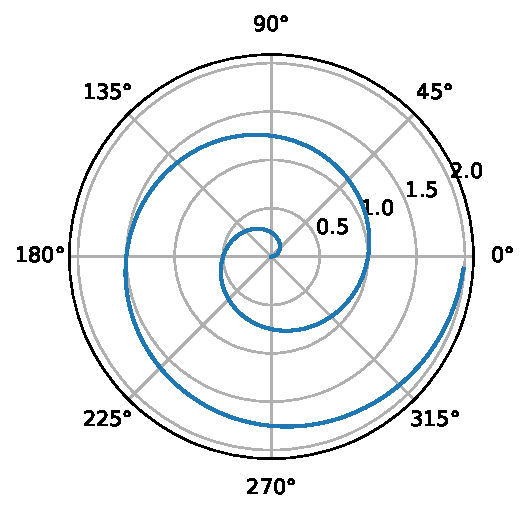
\includegraphics{index_files/figure-pdf/fig-polar-output-1.pdf}

}

\caption{\label{fig-polar}A line plot on a polar axis}

\end{figure}

\hypertarget{experimental-details}{%
\subsubsection{Experimental Details}\label{experimental-details}}

-- TODO: show the results of using the deterministic algorithm vs the
randomized algorithm

\hypertarget{sparsification-of-complete-graphs}{%
\subsection{Sparsification of Complete
Graphs}\label{sparsification-of-complete-graphs}}

\hypertarget{expander-graphs}{%
\subsubsection{Expander Graphs}\label{expander-graphs}}

-- TODO: recap of expanders

-- TODO: expander mixing lemma

\hypertarget{ramanujan-bounds}{%
\subsubsection{Ramanujan Bounds}\label{ramanujan-bounds}}

\hypertarget{the-twice-ramanujan-sparsifier}{%
\subsubsection{The Twice Ramanujan
Sparsifier}\label{the-twice-ramanujan-sparsifier}}

-- TODO: illustration of what happens in the algorithm iteratively on a
complete graph.

\hypertarget{references}{%
\subsubsection{References}\label{references}}

\hypertarget{refs}{}
\begin{CSLReferences}{1}{0}
\leavevmode\vadjust pre{\hypertarget{ref-batson2009twice}{}}%
Batson, Joshua D, Daniel A Spielman, and Nikhil Srivastava. 2009.
{``Twice-Ramanujan Sparsifiers.''} In \emph{Proceedings of the
Forty-First Annual ACM Symposium on Theory of Computing}, 255--62.

\leavevmode\vadjust pre{\hypertarget{ref-benczur1996approximating}{}}%
Benczúr, András A, and David R Karger. 1996. {``Approximating St Minimum
Cuts in {Õ} (n 2) Time.''} In \emph{Proceedings of the Twenty-Eighth
Annual ACM Symposium on Theory of Computing}, 47--55.

\leavevmode\vadjust pre{\hypertarget{ref-cheeger1970lower}{}}%
Cheeger, Jeff. 1970. {``A Lower Bound for the Smallest Eigenvalue of the
Laplacian, Problems in Analysis, a Symposium in Honor of s.''}
\emph{Bochner, Princeton U. Press, Princeton}.

\leavevmode\vadjust pre{\hypertarget{ref-chew1989there}{}}%
Chew, L Paul. 1989. {``There Are Planar Graphs Almost as Good as the
Complete Graph.''} \emph{Journal of Computer and System Sciences} 39
(2): 205--19.

\leavevmode\vadjust pre{\hypertarget{ref-dette1995some}{}}%
Dette, Holger, and William J Studden. 1995. {``Some New Asymptotic
Properties for the Zeros of Jacobi, Laguerre, and Hermite
Polynomials.''} \emph{Constructive Approximation} 11 (2): 227--38.

\leavevmode\vadjust pre{\hypertarget{ref-lee2017sdp}{}}%
Lee, Yin Tat, and He Sun. 2017. {``An Sdp-Based Algorithm for
Linear-Sized Spectral Sparsification.''} In \emph{Proceedings of the
49th Annual Acm Sigact Symposium on Theory of Computing}, 678--87.

\leavevmode\vadjust pre{\hypertarget{ref-rudelson1999random}{}}%
Rudelson, Mark. 1999. {``Random Vectors in the Isotropic Position.''}
\emph{Journal of Functional Analysis} 164 (1): 60--72.

\leavevmode\vadjust pre{\hypertarget{ref-spielman2008graph}{}}%
Spielman, Daniel A, and Nikhil Srivastava. 2008. {``Graph Sparsification
by Effective Resistances.''} In \emph{Proceedings of the Fortieth Annual
ACM Symposium on Theory of Computing}, 563--68.

\leavevmode\vadjust pre{\hypertarget{ref-spielman2004nearly}{}}%
Spielman, Daniel A, and Shang-Hua Teng. 2004. {``Nearly-Linear Time
Algorithms for Graph Partitioning, Graph Sparsification, and Solving
Linear Systems.''} In \emph{Proceedings of the Thirty-Sixth Annual ACM
Symposium on Theory of Computing}, 81--90.

\leavevmode\vadjust pre{\hypertarget{ref-spielman2011spectral}{}}%
---------. 2011. {``Spectral Sparsification of Graphs.''} \emph{SIAM
Journal on Computing} 40 (4): 981--1025.

\leavevmode\vadjust pre{\hypertarget{ref-tat2015constructing}{}}%
Tat Lee, Yin, and He Sun. 2015. {``Constructing Linear-Sized Spectral
Sparsification in Almost-Linear Time.''} \emph{arXiv e-Prints},
arXiv--1508.

\end{CSLReferences}



\end{document}
